\section{Las actividades económicas}

\subsection{La actividad económica}

Las personas, para satisfacer sus necesidades, como la alimentación, el vestido, los servicios (educación, sanidad, etc.), realizan una serie de tareas. A estas tareas las denominamos actividad económica. En esta se distinguen sus \textbf{componentes} (producción, distribución y consumo) y \textbf{quiénes la llevan a cabo} (empresas, familias...).

\subsubsection{Componentes de la actividad económica}

\textbf{Producción}

\vspace{3mm}
Es el conjunto de lo producido para satisfacer nuestras necesidades.

\vspace{3mm}
\textbf{Distribución}

\vspace{3mm}
Es el traslado de los productos producidos hasta las personas que los consumimos.

\vspace{3mm}
\textbf{Consumo}

\vspace{3mm}
Es el uso y disfrute de todo aquello proporcionado por la producción.

\subsubsection{¿Quiénes llevan a cabo la actividad económica?}

\textbf{Empresas}

\vspace{3mm}
Las \textbf{empresas} están formadas por una, varias o muchas personas. Se encargan de producir, distribuir y vender lo que necesitamos. Su fin es obtener beneficios. Se clasifican de distintas formas, como verás en la siguiente doble página.

\vspace{3mm}
\textbf{Personas, familias}

\vspace{3mm}
Las \textbf{personas o familias} son las consumidoras y los consumidores. \textbf{Compran} los bienes para satisfacer sus necesidades. Para ello \textbf{trabajan} en las empresas a cambio de recibir un salario con el que pagan los bienes y servicios que compran.

\subsubsection{¿Qué es necesario? Dinero y tipos de gastos}

Para el pago de productos y bienes que necesitamos, utilizamos el dinero, en forma de billetes o monedas.
En la Antigüedad, el trueque era el sistema utilizado para obtener lo que se necesitaba. Consistía en intercambiar los productos entre sí (gallinas por fruta, vacas por maíz, etc.). Con este sistema era muy difícil fijar el valor de cada producto. La aparición del \textbf{dinero} hizo que el comercio fuera más sencillo y permitió su expansión.

\vspace{3mm}
\textbf{Economía doméstica, nuestra economía}

\vspace{3mm}
Las personas o las familias, cada día, nos enfrentamos a distintos tipos de gastos (Figura \ref{fig:tipos-gastos}) para satisfacer nuestras necesidades, como son los fijos, los variables y los inesperados.

\begin{figure}[!ht]
    \centering
    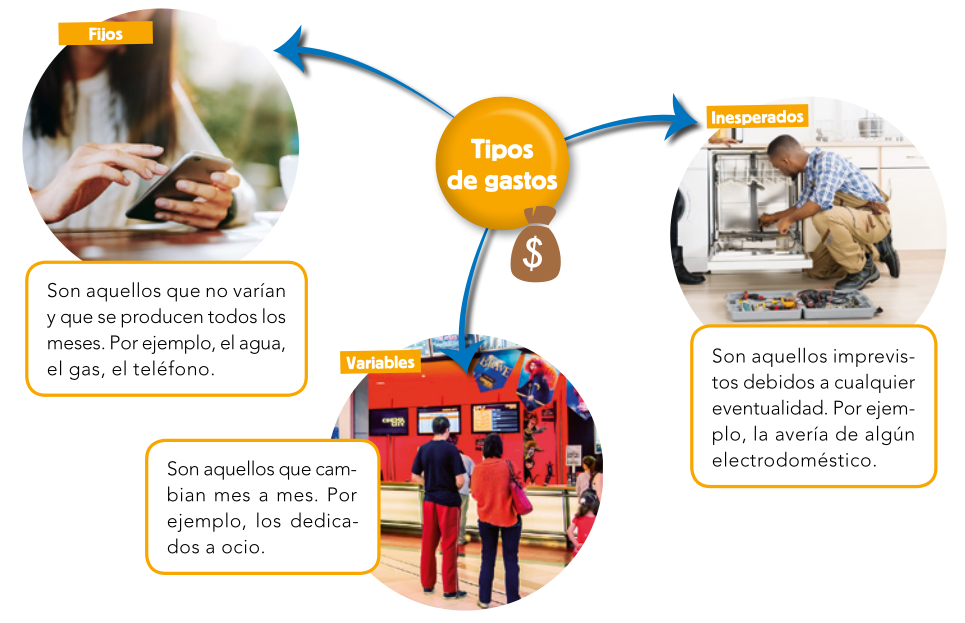
\includegraphics[width=1\linewidth]{Tema4/01_Tipos_gastos.png}
    \caption{Tipos de gastos}
    \label{fig:tipos-gastos}
\end{figure}

\vspace{3mm}
\textbf{Ahorro, publicidad y consumo responsable}

\vspace{3mm}
El \textbf{ahorro} es el dinero que no se destina al gasto y que se guarda para necesidades futuras. La clave del ahorro es la capacidad de juntar dinero de manera regular durante un periodo de tiempo. Antes de adquirir un producto, debemos valorar si realmente lo necesitamos y no dejarnos influenciar siempre por la \textbf{publicidad}, que intenta estimular su compra. Es decir, tenemos que realizar un \textbf{consumo responsable}.

\subsection{Las empresas y sus tipos}

Como ya has visto, las empresas se encargan de producir, distribuir y vender lo que necesitamos. Se pueden clasificar de muchas maneras: por su tipo de actividad (Figura \ref{fig:empresas-actividad}), por el lugar de donde procede el capital con el que se crean (Figura \ref{fig:empresas-capital}), por su tamaño (Figura \ref{fig:empresas-tamaño}), etc.

\begin{figure}[!ht]
    \centering
    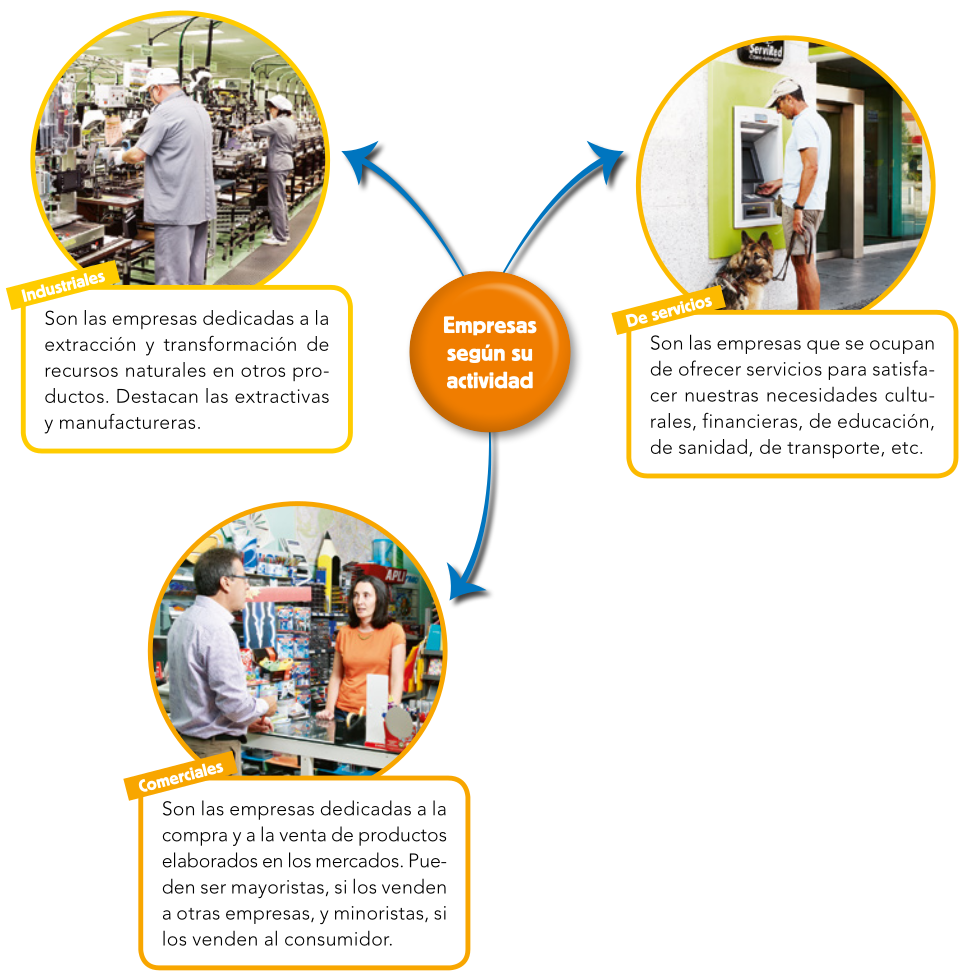
\includegraphics[width=0.8\linewidth]{Tema4/02_Empresas_actividad.png}
    \caption{Empresas según su actividad}
    \label{fig:empresas-actividad}
\end{figure}

\begin{figure}[!ht]
    \centering
    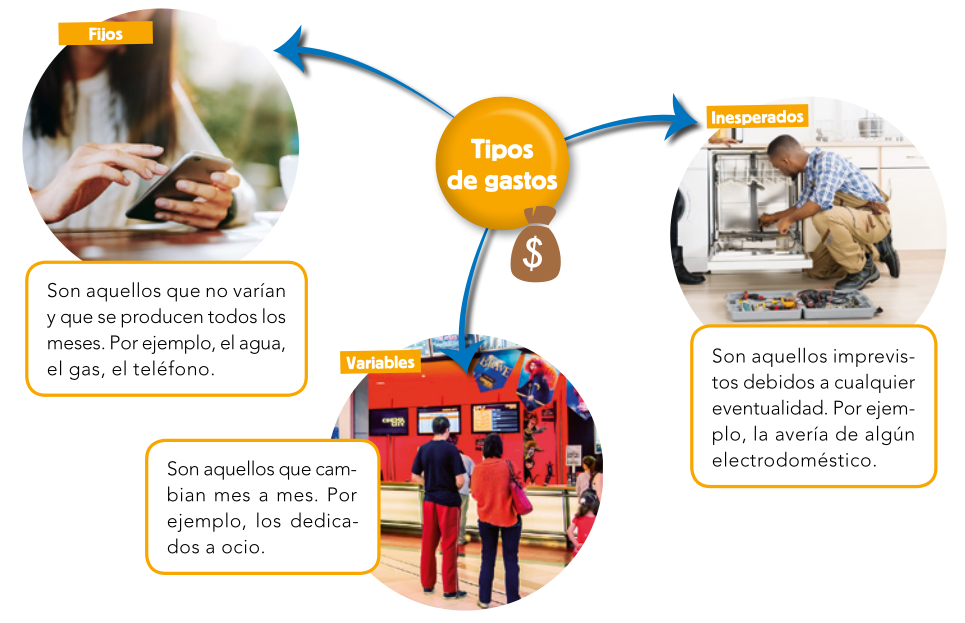
\includegraphics[width=0.8\linewidth]{Tema4/01_Tipos_gastos.png}
    \caption{Empresas según de donde procede el capital}
    \label{fig:empresas-capital}
\end{figure}

\begin{figure}[!ht]
    \centering
    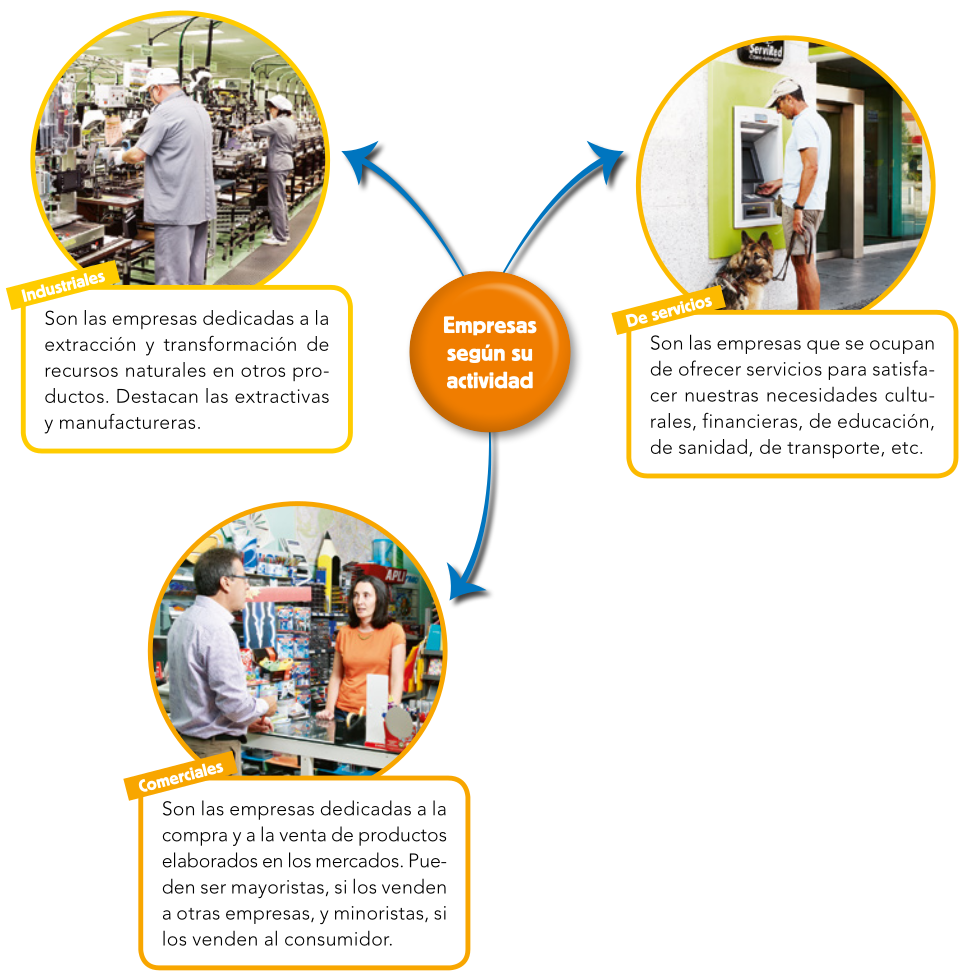
\includegraphics[width=0.8\linewidth]{Tema4/02_Empresas_actividad.png}
    \caption{Empresas según su tamaño}
    \label{fig:empresas-tamaño}
\end{figure}

\subsection{Sectores económicos. Sector primario}